\begingroup
\renewcommand{\arraystretch}{1.45}
\fancyhead[L]{\small ZUR THEORIE DER NEUEN TRANSZENDENTEN. V.}

\Needspace{18\baselineskip}
\par\medskip\Needspace{5\baselineskip}\pdfbookmark[1]{Art. 12}{transscendentes-v-art-12}\centerline{[12.]}\nobreak\smallskip
\textsc{Theorem.} Wenn der imaginäre Teil von \(t\) und \(\frac1t\) zwischen \(-i\) und
\(+i\) liegt, so ist der reelle Teil von
\[
\left(\frac{Qt}{Pt}\right)^2
\]
positiv.

\noindent\begin{minipage}{.45\linewidth}
Geometrisch zu beweisen
\end{minipage}\hfill
\resizebox{.47\linewidth}{!}{\begin{tikzpicture}[x=1bp,y=-1bp,line cap=round,line join=round]
\path[use as bounding box] (0,0) rectangle (770,270);
\begin{pgfinterruptboundingbox}
\draw[line width=2.5bp] (85,73) -- (727,73);
\draw[line width=2.5bp] (86,221) -- (184,221);
\draw[line width=2.5bp] (251,221) -- (728,221);
\draw[line width=2.5bp] (92,81) -- (91,213);
\draw[line width=2bp] (101,85) .. controls (112,109) and (115,129.0) .. (100,141.0);
\draw[line width=2bp] (100,151.0) .. controls (115,168.0) and (112,187) .. (101,208);
\node[inner sep=0pt,outer sep=0pt,rotate=0] at (72,52) {\scalebox{4}{\ensuremath{i}}};
\node[inner sep=0pt,outer sep=0pt,rotate=0] at (247,38) {\scalebox{4}{\ensuremath{1+i}}};
\node[inner sep=0pt,outer sep=0pt,rotate=0] at (62,140) {\scalebox{4}{\ensuremath{0}}};
\node[inner sep=0pt,outer sep=0pt,rotate=0] at (386,147) {\scalebox{3.65}{\textbf{Bereich für }$t$\textbf{ und }$\dfrac1t$}};
\end{pgfinterruptboundingbox}
\end{tikzpicture}
}


\Needspace{20\baselineskip}
Unter dieser Bedingung ist also das arithmetisch-geometrische Mittel zwischen
\[
\mu P(\tfrac12t)^2\qquad\qquad\mu Q(\tfrac12t)^2
\]
indem man immer das geometrische Mittel zwischen \(m,n\) so nimmt, dass
\(\frac{\surd mn}{m}\) einen positiven reellen Teil hat,
\[
=\mu
\]
Ein solches Mittel nennen wir das einfachste Mittel.


\Needspace{26\baselineskip}
Ist das einfachste AG.\ Mittel zwischen \(m,n,=\mu\), das zwischen
\(m,\surd(mm-nn),=\frac\mu t\), so ist \(t\) der Kanon des Verhältnisses
\(\frac nm\), nämlich

\SourceLeaf{487}
\[
\frac mn=\left(\frac{Qt}{Pt}\right)^2
\]
dann ist das einfachste AG.\ Mittel zwischen \(m\) und \(-n\)
\[
=\frac\mu{1+2it}
\]
und der dazu gehörige Kanon
\[
=\frac t{1+2it}=\frac1{\frac1t+2i}
\]


\Needspace{19\baselineskip}
Die Gleichung
\[
\left(\frac{Qt}{Pt}\right)^2=A
\]
hat immer eine und nur eine Lösung in dem Bereich
\begin{center}
\resizebox{.48\linewidth}{!}{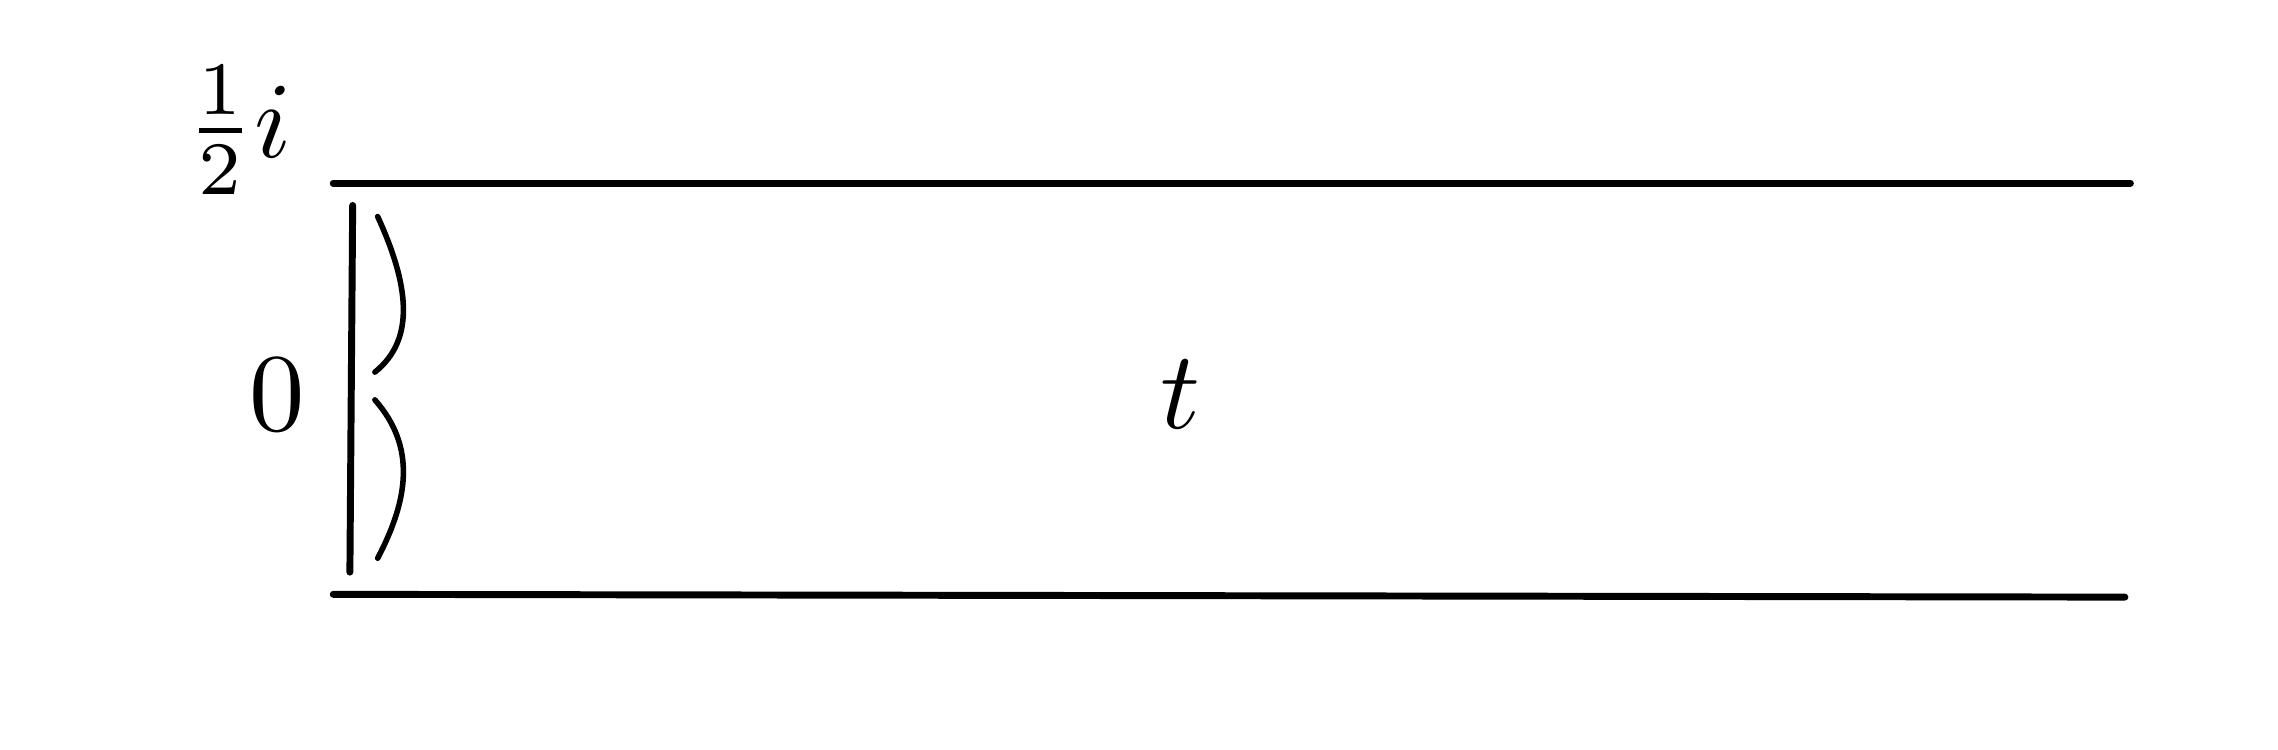
\begin{tikzpicture}[x=1bp,y=-1bp,line cap=round,line join=round]
\path[use as bounding box] (0,0) rectangle (800,250);
\begin{pgfinterruptboundingbox}
\draw[line width=2.5bp] (110,56) -- (757,56);
\draw[line width=2.5bp] (110,204) -- (755,205);
\draw[line width=2.5bp] (117,64) -- (116,196);
\draw[line width=2bp] (126,68) .. controls (137,92) and (140,112.0) .. (125,124.0);
\draw[line width=2bp] (125,134.0) .. controls (140,151.0) and (137,170) .. (126,191);
\node[inner sep=0pt,outer sep=0pt,rotate=0] at (76,37) {\scalebox{3.9}{\ensuremath{\frac12 i}}};
\node[inner sep=0pt,outer sep=0pt,rotate=0] at (90,132) {\scalebox{4}{\ensuremath{0}}};
\node[inner sep=0pt,outer sep=0pt,rotate=0] at (415,132) {\scalebox{4}{\ensuremath{t}}};
\end{pgfinterruptboundingbox}
\end{tikzpicture}
}
\end{center}


\Needspace{17\baselineskip}
Es sei \(\alpha\delta-\beta\gamma=1,\)
\(\alpha\equiv\delta\equiv1\ (\mathrm{mod.}\,4),\)
\(\beta,\gamma\) gerade
\[
t'=i\frac{\alpha t+\beta i}{\gamma t+\delta i}
\]
dann ist
\[
\left(\frac{Qt'}{Pt'}\right)^2=i^\gamma\left(\frac{Qt}{Pt}\right)^2
\]


\Needspace{28\baselineskip}
\par\medskip\Needspace{5\baselineskip}\pdfbookmark[1]{Art. 13}{transscendentes-v-art-13}\centerline{[13.]}\nobreak\smallskip
Fünfteilung
\[
\begin{array}{ll}
a&A\\[8pt]
b&B\\[8pt]
c=\surd(aa-bb)&C=\surd(AA-BB)
\end{array}
\]
\[
2v=-aA+bB+cC
\]
\[
4v=aa-6aA+5AA=-(bb-6bB+5BB)=-(cc-6cC+5CC)
\]
\[
v=-A\surd(AA+v)+B\surd(BB-v)+C\surd(CC-v)
\]


\Needspace{18\baselineskip}
\SourceLeaf{488}

Wendet man die Elimination auf eine Gleichung
\[
\surd a+\surd b+\surd c+\surd d=0
\]
an, so ergibt sich
\[
0=\Sigma(a^4-4a^3b-2aabb+4aabc-24abcd)
\]


\Needspace{19\baselineskip}
\par\medskip\Needspace{5\baselineskip}\pdfbookmark[1]{Art. 14}{transscendentes-v-art-14}\centerline{[14.]}\nobreak\smallskip
Die $7^{\mathrm{plication}}$ beruht auf
\[
\begin{gathered}
\relax[a\sin(\varphi+A)+b\sin(3\varphi+B)]^2\sin(\varphi+k)\\[8pt]
=\alpha\sin(\varphi+l)
 +\beta\sin(3\varphi+l)
 \\[8pt]\quad{}+\gamma\sin(5\varphi+l)+\delta\sin(7\varphi+l)
\end{gathered}
\]


\Needspace{28\baselineskip}
\par\medskip\Needspace{5\baselineskip}\pdfbookmark[1]{Art. 15}{transscendentes-v-art-15}\centerline{[15.]}\nobreak\smallskip
Bei der Dreiteilung setzt man
\[
\surd\frac{q}{p}=n,\qquad \surd\frac{Q}{P}=N
\]
und erhält
\[
\frac{N^{4}
 -n^{4}}{1-nnNN}
 =2nN,\qquad
\frac{ppQQ-qqPP}{pP-qQ}=2\surd pPqQ
\]

proportional
\begingroup\small\setlength{\arraycolsep}{1.5pt}\[
\begin{array}{c|l||c|l||c|l}
p^4&3\cos\varphi\sin\varphi^3
&q^4&3\cos(60^0-\varphi)\sin(60^0-\varphi)^3
&r^4&3\cos(120^0-\varphi)\sin(120^0-\varphi)^3\\[8pt]
P^4&\cos\varphi^3\sin\varphi
&Q^4&\cos(60^0-\varphi)^3\sin(60^0-\varphi)
&R^4&\cos(120^0-\varphi)^3\sin(120^0-\varphi)
\end{array}
\]\endgroup

\clearpage
\endgroup
